\section{Recherche du chemin le plus court}

Il n'y a pas d'alternative, si on veut trouver le chemin le plus court ; il faut essayer toutes les solutions. Mais il existe une alternative intéressante qui permet d'éviter un grand nombre de calculs inutile. Reprenons l'arbre binaire crée précédemment en prenant soin de garder en mémoire le \textit{Tree} contenant la sortie ainsi que les \textit{Tree} finaux représenté par des ronds rouges pleins.

\begin{figure}[!h]
\centering
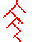
\includegraphics[width=0.4\textwidth]{5.recherche/tree.pdf}
\caption{Arbre binaire avec les \textcolor[rgb]{0.91,0.91,0}{bonbons} et les \textcolor[rgb]{0.5,0,1}{monstres}.}
\end{figure}

Parcourons chaque \textit{Tree} final et remontons l'arbre jusqu'à un \textit{Tree} possédant soit la sortie, soit un bonbon, soit un autre fils et en supprimant les autres \textit{Tree} inutiles c-à-d ceux qui ne contiendrait rien ou un monstre.

\begin{figure}[!h]
\centering

\includegraphics[width=0.4\textwidth]{5.recherche/treeStepDelete.pdf}
\caption{Simplification de l'arbre binaire étape par étape.}
\end{figure}

Ainsi l'arbre binaire se simplifie et devient nettement plus clair.

\begin{figure}[!h]
\centering
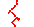
\includegraphics[width=0.4\textwidth]{5.recherche/treeSimplification.pdf}
\caption{Arbre binaire simplifié.}
\end{figure}

Il nous reste plus qu'à remonter du \textit{Tree} de sortie jusqu'à la racine (l'entrée) et de compter le nombre de bonbon on a besoin. Ici on croise 2 monstres et 1 bonbon, il nous manque donc 1 bonbon pour arriver à la sortie.

\begin{figure}[!h]
\centering
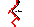
\includegraphics[width=0.4\textwidth]{5.recherche/treeSearch.pdf}
\caption{Recherche du nombre de bonbon qu'on a besoin.}
\end{figure}

Ensuite nous pouvons faire le parcours récursif depuis la racine en autorisant autant de demi tour que de bonbon manquant. Ici, un bonbon est manquant donc on a droit qu'à un seul demi tour lorsqu'on arrive à un \textit{Tree} final. On remarque que le parcours récursif est beaucoup plus rapide que si nous avions pas fait les simplifications.